\chapter{App}
\section{Registrierung}
Bei der Registrierung gibt der Benutzer seinen gewünschten Benutzernamen und sein Passwort ein. Der Benutzername und der SHA1-Hash des Passworts wird dann an den Server gesendet und sofern der Benutzername nicht bereits existiert wird der neue Benutzer angemeldet. Dies wird dem Benutzer mit einer Nachricht mitgeteilt. Der Benutzer kann sich nun anmelden.

\begin{capfigure}[App - Registrierung]
	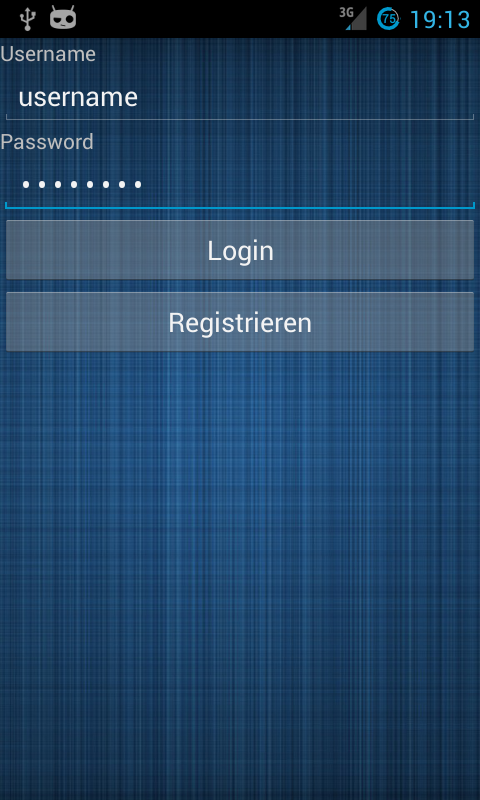
\includegraphics[width=6cm]{images/app/login}
\end{capfigure}


\section{Anmeldung}
Ein bereits registrierter Benutzer kann sich analog zur Registrierung anmelden. War die Anmeldung erfolgreich bekommt die App ein Token und wechselt in das Hauptmenü.

\section{Hauptmenü}
\TODO{TG: machen}

\begin{capfigure}[App - Hauptmenü]
	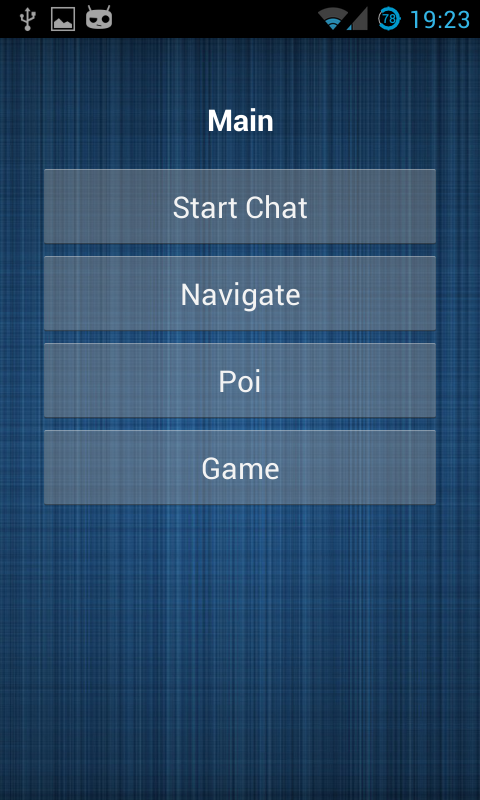
\includegraphics[width=6cm]{images/app/main_menu}
\end{capfigure}

\section{Chatsystem}
Um den Nutzern der App die Möglichkeit zu bieten miteinander zu kommunizieren wurde ein Nachrichtensystem implementiert. Dieses ermöglicht es den Nutzern der App über diese miteinander zu kommunizieren und ermöglicht es Freunde zur Freundesliste hinzuzufügen. 
Die Kommunikation erfolgt über den zentralen Server. Alle gesendeten Nachrichten eines Nutzers werden dort gespeichert und können von den Kommunikationspartnern abgerufen werden. Somit ist es kein Problem Nachrichten zu empfangen, wenn man zum Zeitpunkt des Sendens nicht online war. Neben den Nachrichten wird auch die Freundesliste auf dem Server abgelegt.
Startet man die Nachrichtenfunktion, so erhält man zunächst die Möglichkeit neue Freunde (andere regstrierte Benutzer) durch Eingabe deren Namen zur Freundesliste hinzuzufügen. In der selben Ansicht wird die Freundesliste angezeigt. 
\TODO Screenshot "friendlist"
Durch Tippen auf einen Freund in der Liste öffnet man die Kommunikationsansicht. Dort werden bereits versendete und empfangene Nachrichten angezeigt. Hier lassen sich dann Nachrichten eingeben und durch antippen von "Nachricht senden" übertragen. Je Nachdem ob man Empfänger oder sender ist wird die Nachricht Farbig dargestellt.
\TODO Screenshot "chat"
Dank dieser Funktionalität wird es den Nutzern der App ermöglicht auf einfache Art und Weise Kontaktpflege zu betreiben und sich beispielsweise für ein Treffen bei einem der POI's zu verabreden. Dank der integrierten Nachrichtenlösung ist es möglich, dass sich die Nutzer verständigen können ohne irgendwelche persönlichen Daten veröffentlichen zu müssen.

\section{Kompass}
Neben dem Kompass werden in der KompassView noch weitere Daten dargestellt. Es wird die aktuelle GPS-Position in Form von Longitude und Latitude angezeigt.

\begin{capfigure}[App - Kompass]
	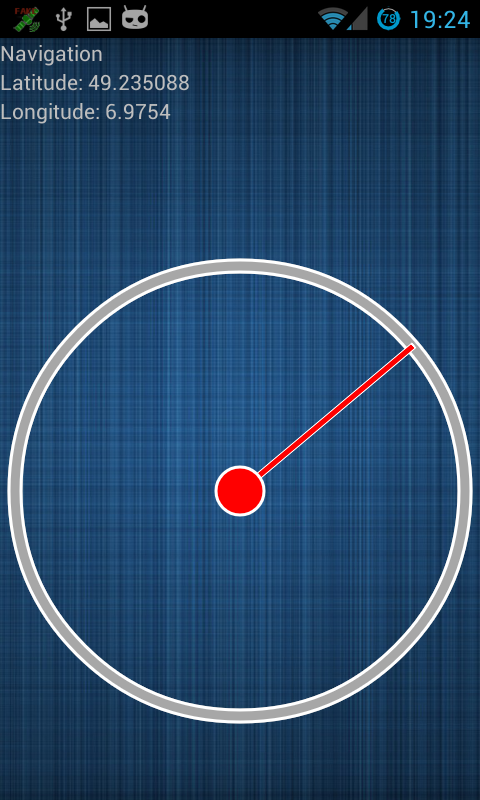
\includegraphics[width=6cm]{images/app/compass}
\end{capfigure}

\section{Navigation}
Für die Navigation wird die KompassView verwendet. Wenn sich die KompassView im Navigationsmodus befindet wird zusätzlich die Richtung zum Ziel als auch die Entfernung angezeigt.

\begin{capfigure}[App - Navigation]
	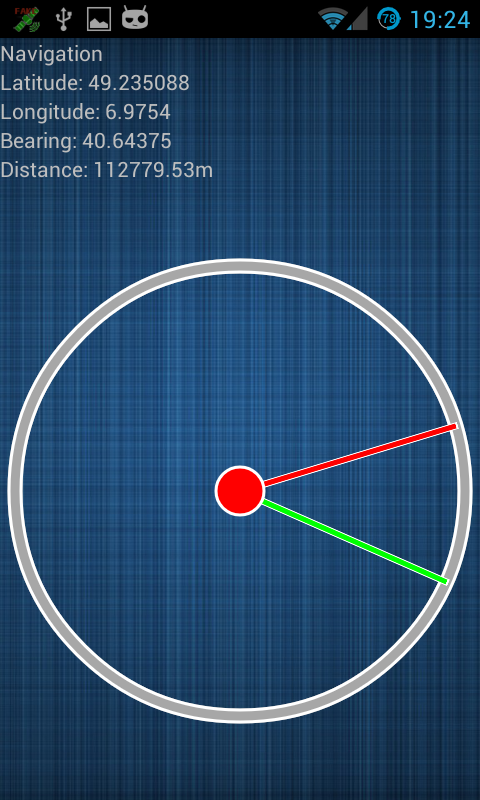
\includegraphics[width=6cm]{images/app/navigation}
\end{capfigure}

Für die Navigation wird auf Funktionen des Android-Frameworks zurückgegriffen. Über diese Funktionen wird die Distanz berechnet und das Bearing. Bearing gibt den Winkel zum Nordpol an.

\section{POIs}
Die App verbindet POI's (point of interest)  mit bestimmten Ereignissen wie einem Spiel. Ein POI besteht im Wesentlichen aus Koordinaten, Namen und Eigenschaft.  Die POI's werden ebenfalls in der Datenbank gespeichert und können über den Punkt "POI" aus dem Hauptmenü aufgerufen werden. Wählt man einen POI aus der Liste durch antippen aus, werden einem die Details angezeigt wie in folgender Abbildung zu sehen ist.
\TODO Screenshot POI Liste
Dazu gehören neben Längengrad, Breitengrad und Namen des POI's auch die Distanz zum POI in Metern angezeigt. Mit dem Button "Navigiere zu POI" wird die Navigation welche zuvor beschrieben wurde aufgerufen.

\section{Spiele}

\TODO{TG: Anzeige der Spiele machen}

\subsection{Rock, Paper, Scissors, Lizzard, Spock}
Nachdem man sich für das Spiel angemeldet hat wartet die App bis ein anderer Spieler bereit ist. Sobald beide Spieler bereit sind erscheinen die Buttons zur Auswahl der zu spielenden Hand. Haben beide Spieler ihre Hand gewählt wird das Ergebnis angezeigt.

\begin{capfigure}[App - Rock, Paper, Scissors, Lizzard, Spock]
	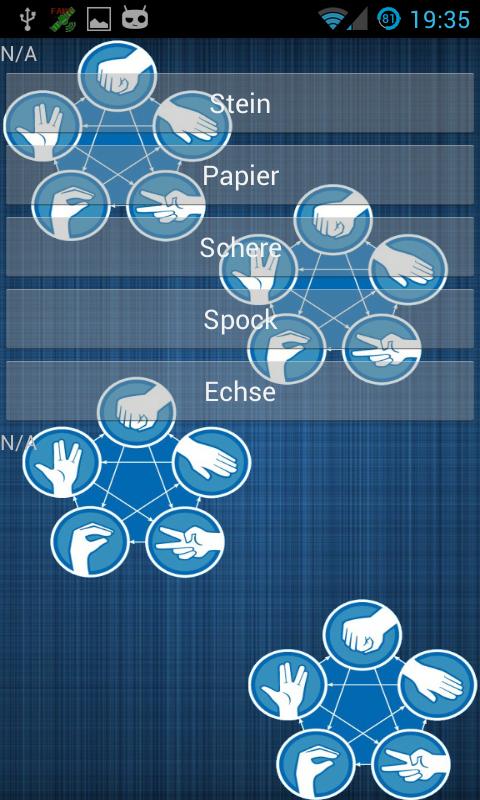
\includegraphics[width=6cm]{images/app/rpssl}
\end{capfigure}



\subsubsection{Spielablauf}
\TODO{Im Details beschreiben wie ein Spiel erzeugt wird und gespielt wird}

